\section{Introduction to MRI}

\begin{frame}[plain,c]
    %\frametitle{A first slide}
    
    \begin{center}
        \color{DarkBlue}
    \Huge Magnetic Resonance Imaging~(MRI)
    \end{center}
    
\end{frame}

\begin{frame}{What does an MRI look like?}
    \begin{figure}
        \centering
        \begin{subfigure}{0.45\textwidth}
            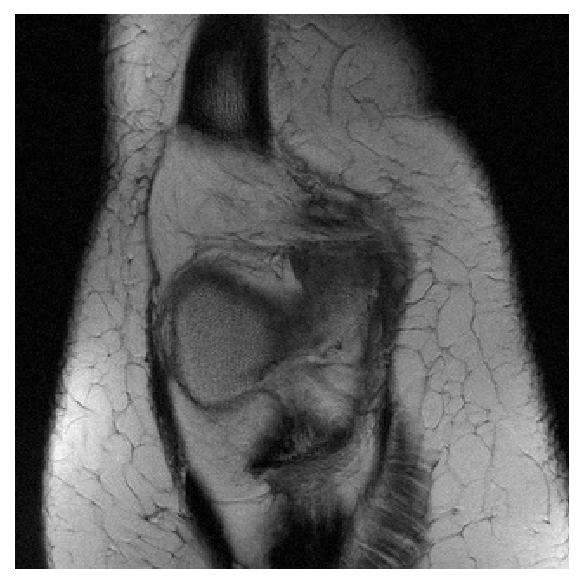
\includegraphics[height=0.6\textheight]{Figures/intro_figures/example_knee_fastmri.pdf}
        \end{subfigure}
        \begin{subfigure}{0.45\textwidth}
            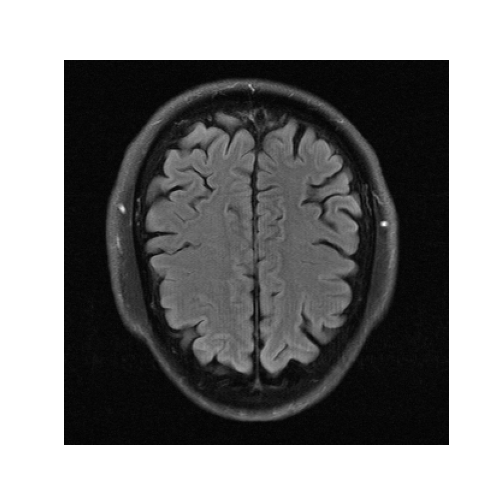
\includegraphics[height=0.6\textheight]{Figures/intro_figures/brain_mri.png}  
        \end{subfigure}
        \caption{\label{fig:mri-example} \textbf{Examples of MR images}: knee and brain taken from the fastMRI dataset.\footfullcite{Zbontar}}
    \end{figure}
    % explain content of image: it's not a photo, but it tells us the tissue density
    % explain that MRI is non invasive an high res!
\end{frame}



% MRI is so popular why isnt it solved already ?
\begin{frame}{MRI players}
    \begin{center}
        \begin{tikzpicture}[
            >=stealth,font=\Large, node distance=2em,
            b0/.style={line width=7pt, draw=DarkGreen},
        ]
            % nodes
            \node[] (mri) {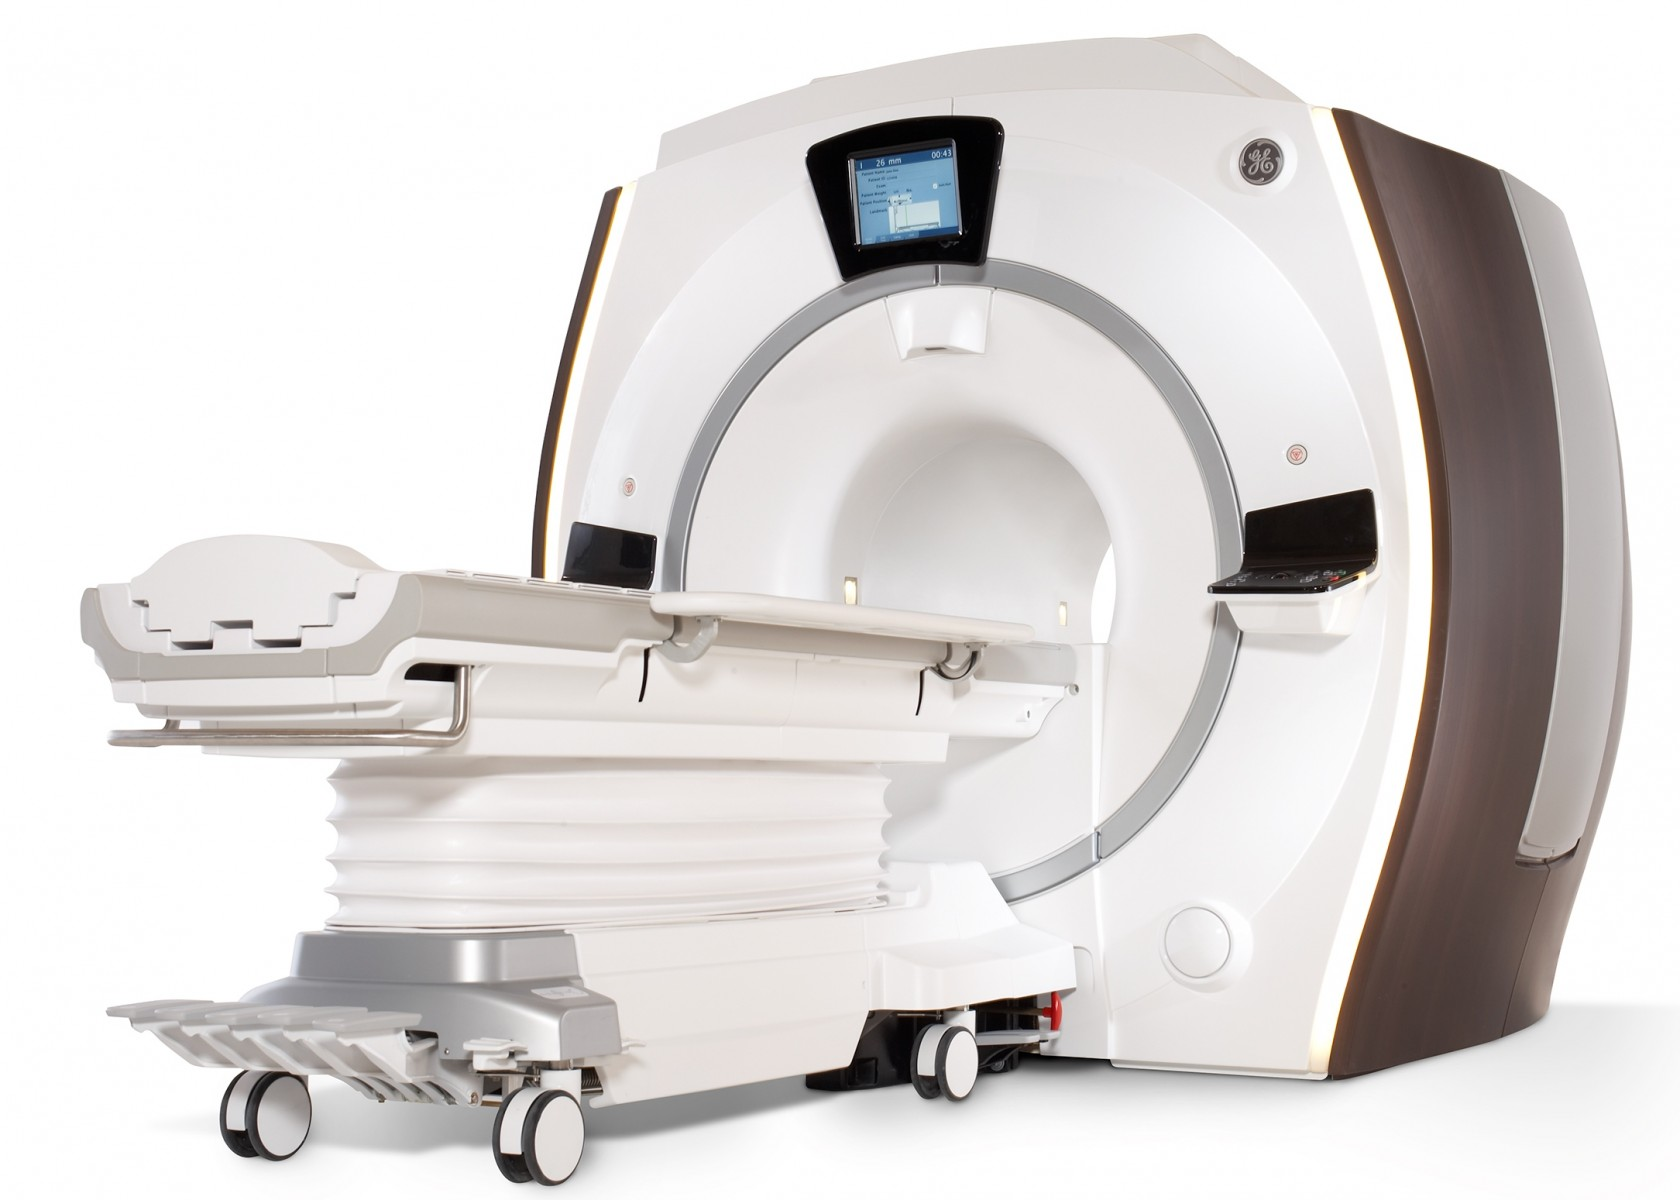
\includegraphics[height=0.3\textheight,]{Figures/intro_figures/mri.jpg}};
            \node[below=of mri] (brain) {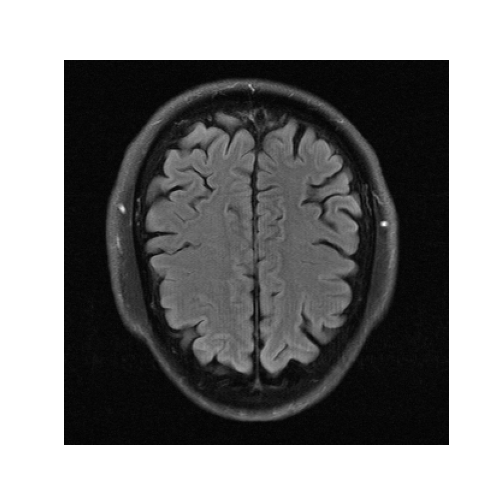
\includegraphics[height=0.3\textheight,angle=180]{Figures/intro_figures/brain_mri.png}};
            \shade[ball color = blue!47, visible on=<3>] ($(brain.east)+(8cm,0)$) circle (1cm);
            \node[visible on=<3>] at ($(brain.east)+(8cm,-1.3cm)$) {Proton};
            \node[visible on=<2->] (bottom_arrow) at ($(mri.east)+(7.5cm,-1.3cm)$) {$\Bb_0$};
            % arrows
            %% pointing
            %% field
            \draw[->,-{Triangle[width=18pt,length=9pt]}, b0, visible on=<2->]  ($(mri.east)+(7.5cm,-1cm)$) -- ($(mri.east)+(7.5cm,1cm)$);
            \draw[->, visible on=<2->] (mri.east) --  ($(mri.east)+(7cm,0)$);
            \draw[->, visible on=<3>] (brain.east) --  ($(brain.east)+(6.5cm,0)$);
        \end{tikzpicture}
    \end{center}
\end{frame}


\begin{frame}{Nuclear Magnetic Resonance}
    \begin{center}
        \begin{tikzpicture}[
            >=stealth,font=\Large, node distance=2em,
            b0/.style={line width=7pt, draw=DarkGreen},
            spin/.style={line width=2pt},
            excit/.style={line width=8pt},
            pulse/.style={line width=3pt, color=blue!87},
            pulse_text/.style={above,midway,color=blue!87},
        ]
            % nodes
            \shade[ball color = blue!47] (0,0) circle (1cm);
            \node(top_spin) at (0,1cm) {};
            \node(bottom_spin) at (0,-1cm) {};
            \node(top_arrow) [above=of top_spin] {};
            \node(bottom_arrow) [below=of bottom_spin] {$\Bb_0$};
            \node(coil) [circle, draw, visible on=<3>] at (4.5cm,0) {\textbf{Antenna}};
            % arrows/lines
            \draw[->,-{Triangle[width=18pt,length=9pt]}, b0] (top_spin.south) -- (top_arrow);
            \draw[b0] (0,-1cm) -- (bottom_arrow);
            \begin{scope}[on background layer]
                \draw<1>[->,dashed,semithick] (-0.6cm,1.6cm) arc [start angle=180, end angle=-70, x radius=0.6cm, y radius=.1cm];                
            \end{scope}
            %% excitation/relaxation
            \draw[excit, visible on=<2>, color=red!87,->] (-1.6cm,1.6cm) arc [start angle=95, end angle=175, x radius=1.6cm, y radius=1.6cm] node [left,midway, color=red!87, xshift=-0.3cm] {\textbf{Excitation}};
            \draw[excit, visible on=<3>, color=green!87, <-] (-1.6cm,1.6cm) arc [start angle=95, end angle=175, x radius=1.6cm, y radius=1.6cm] node [left,midway, color=green!87, xshift=-0.3cm] {\textbf{Relaxation}};
            %% pulses
            \draw[<-, pulse,visible on=<2>] (1.9cm,0cm) -- node [pulse_text] {\textbf{RF pulse}} ($(coil.west)+(-0.3cm,0)$);
            \draw[->, pulse,visible on=<3>] (1.9cm,0cm) -- node [pulse_text] {\textbf{FID}} ($(coil.west)+(-0.3cm,0)$);
            %% arrow spin
            \draw<1,3>[->,spin] (-0.3cm,0.8cm) -- (-0.6cm,1.6cm);
            \draw<2>[->,spin] (-0.9cm,0.cm) -- (-1.8cm,0cm);
            \begin{scope}[on background layer]
                \draw<1,3>[spin] (0.3cm,-0.8cm) -- (0.6cm,-1.6cm);
                \draw<2>[spin] (0.9cm,0cm) -- (1.8cm,0cm);
            \end{scope}
            
        \end{tikzpicture}
    \end{center}
\end{frame}

\begin{frame}{Physics of MRI - 2}
    % Signal equation $\Rightarrow$ k-space
    % The \textbf{k-space} vector, $\kb(t) = \frac{\gamma}{2\pi} \int_0^t \Gb(\tau) \dif \tau$, defines how we traverse the Fourier space of the anatomical image.
    \textbf{k-space} vector: $\kb(t) = \frac{\gamma}{2\pi} \int_0^t \Gb(\tau) \dif \tau$.

    % We are sampling in the Fourier space of the anatomical image
    %     \caption{\label{fig:example-kspace}\textbf{Example of a k-space with its corresponding anatomical image}: The raw data is from the fastMRI dataset. The k-space is in log-scale and only the magnitude of the 2 images are represented. We selected only a single coil from the 16 coils available for illustrative purposes.}

    \begin{center}
        \begin{tikzpicture}
            \node (kspace) {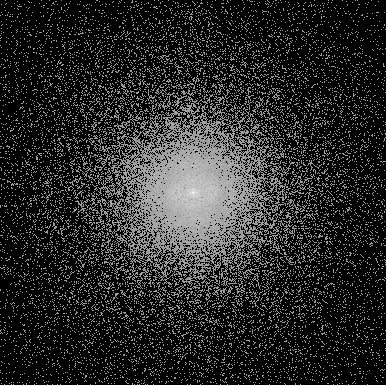
\includegraphics[width=0.31\textwidth]{Figures/intro_figures/kspace_phantom.png}};
            \node[below=0.7em of kspace] (kspace_exp) {$\kb(t) \mapsto S_{tr}(t)$};
            \node[right=of kspace] (brain) {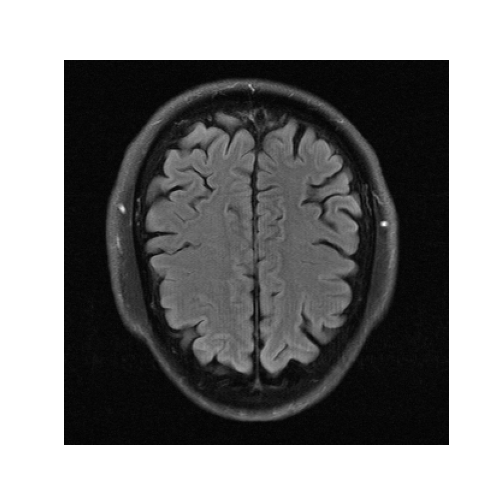
\includegraphics[width=0.4\textwidth, angle=180]{Figures/intro_figures/image_gt (2).png}};
            \node[below=-1em of brain] (brain_exp) {$\propto \rho(\rb)$};
            \draw[-{Triangle[width=18pt,length=8pt]}, line width=10pt, draw=blue!57](kspace.east) -- node [midway,above] {IFFT} ($(brain.west)+(1.6em, 0)$);
        \end{tikzpicture}
    \end{center}
\end{frame}

\begin{frame}{Physics of MRI - 3}
    % Let's not forget our initial goal here: we want to understand why MRI is slow
    % The relaxation is slow !
    \begin{block}{Recap}
        MRI relies on the nuclear magnetic resonance phenomenon. This enables us to sample the Fourier space of the anatomical object of interest.
    \end{block}
    \pause
    MRI is slow, because the \textbf{relaxation} is slow!
\end{frame}

\begin{frame}{Where is there room for acceleration?}
    % Explain the concept of redundancy
    % first example: partial Fourier $\Rightarrow$ give limits
    % \textbf{Redundancy}, otherwise called \textbf{sparsity, symmetry, structure or a priori information}, is the core concept that will help us accelerate MRI.\\
    \textbf{Redundancy}, or \textbf{sparsity, symmetry, structure or a priori information}, is the key.\\
    
    % \begin{overprint}
    %     \onslide<2>
    %     \hfill \break
    % % Here is an illustrative example:
    % An illustrative example:
    % \begin{figure}
    %     \centering
    %     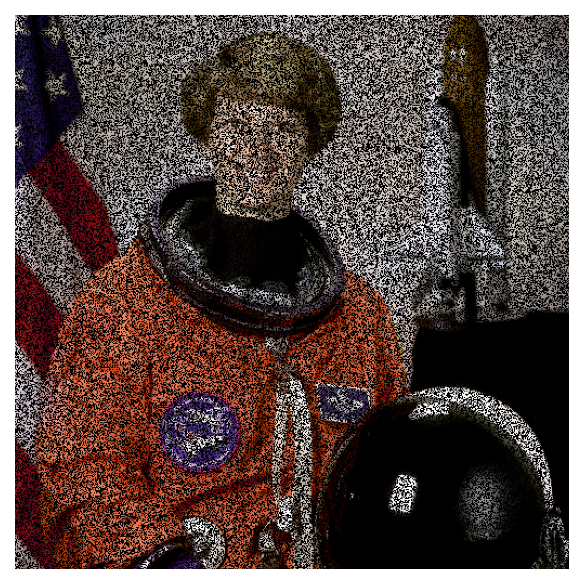
\includegraphics[height=0.4\textheight]{Figures/intro_figures/astronaut_masked.pdf}
    %     \caption{\label{fig:astronaut-masked}\textbf{The inpainting problem.} 
    %     % Even without access to all the pixel values directly, we can infer them, because the information in the image is redundant.
    %     }
    % \end{figure}
    
    % \onslide<3>
    % \hfill \break
    % An illustrative example:
    % \begin{figure}
    %     \centering
    %     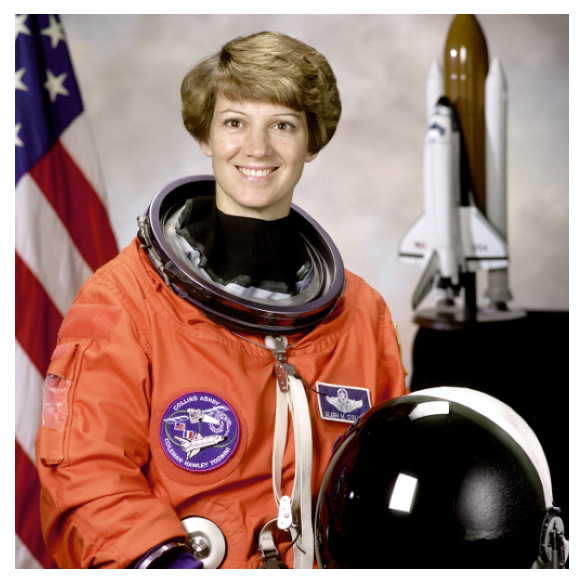
\includegraphics[height=0.4\textheight]{Figures/intro_figures/astronaut.pdf}
    %     \caption{\label{fig:astronaut}\textbf{The inpainting problem.} 
    %     % Even without access to all the pixel values directly, we can infer them, because the information in the image is redundant.
    %     }
    % \end{figure}
    
    % \onslide<4>
    \pause
        \hfill \break
        Where is it in MRI?

        % Yes! The anatomical image is real-valued so its Fourier Transform~(FT) has a conjugate symmetry.
        Fourier Transform~(FT) has a conjugate symmetry $\Rightarrow$ \textbf{Partial Fourier}
        % Using this redundancy to sample less points in the k-space (i.e. using the relaxation fewer times) is a technique called \textbf{Partial Fourier}.
        
        % But in practice it is still needed to sample 6/8 of the Fourier space (acceleration of 1.3).\footfullcite{emri}
        Resulting acceleration: 1.3
    
    % \end{overprint}
    
\end{frame}

\begin{frame}{Parallel imaging}
    % "forging" the redundancy
    % We can build more redundancy in the measuring system by using \textbf{more antennas (called coils)} to measure the magnetic signal.
    More redundancy using \textbf{more antennas (called coils)} $\Rightarrow$ \textbf{Parallel Imaging~(PI)}
     
    % This technique is called \textbf{Parallel Imaging~(PI)}. 
    % A reconstruction algorithm is now needed to handle the multi-coil undersampled data.
        % \textbf{SENSE}\footfullcite{Pruessmann1999SENSE:MRI} and \textbf{GRAPPA}\footfullcite{Griswold2002GeneralizedGRAPPA} are such algorithms.    
    Multi-coil reconstruction algorithms: \textbf{SENSE}\footfullcite{Pruessmann1999SENSE:MRI} and \textbf{GRAPPA}\footfullcite{Griswold2002GeneralizedGRAPPA}.
    % GRAPPA + SENSE examples
\end{frame}

\begin{frame}{The example of GRAPPA}
    \begin{figure}
        \centering
        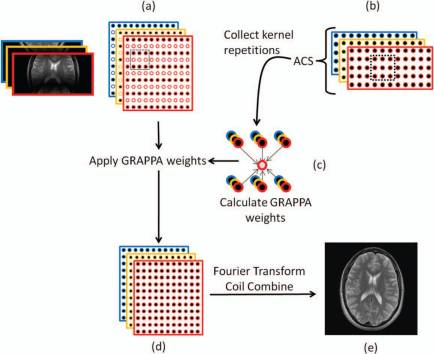
\includegraphics[height=0.6\textheight]{Figures/intro_figures/GRAPPA.jpeg}
        \caption{\label{fig:GRAPPA}\textbf{GRAPPA illustration.} Image courtesy of \citet{deshmane2012parallel}.
        }
    \end{figure} 
\end{frame}

\begin{frame}{Limits of Parallel Imaging}
    % Max AF
    Resulting acceleration: 2
    % ow: https://www.siemens-healthineers.com/magnetic-resonance-imaging/options-and-upgrades/clinical-applications/syngo-grappa says 2,3
\end{frame}